% Conference slides (20-25 min): Sensitivity, Informativeness, and
% Misspecification in GMM Estimation. Figures live in slides/fig/.
% Sparse, equation-first; propositions stated formally; assumptions in the
% appendix with back-and-forth hyperlinks.
\documentclass[11pt,aspectratio=169]{beamer}

\usetheme{default}
\usecolortheme{seahorse}
\setbeamertemplate{navigation symbols}{}
\setbeamertemplate{footline}[frame number]
\setbeamertemplate{itemize items}[circle]
\setbeamercolor{frametitle}{fg=black!85}
\setbeamerfont{frametitle}{series=\bfseries,size=\large}
\setbeamercolor{alerted text}{fg=blue!60!black}

\setbeamertemplate{theorems}[numbered]
\setbeamercolor{block title}{bg=blue!14,fg=black!88}
\setbeamercolor{block body}{bg=blue!4}
\newtheorem{prop}{Proposition}
\newtheorem{defn}{Definition}
\newtheorem{coro}{Corollary}

\usepackage{amsmath,amssymb,bm}
\usepackage{graphicx}
\graphicspath{{fig/}}
\usepackage{booktabs}

\newcommand{\E}{\mathbb{E}}
\newcommand{\Var}{\operatorname{Var}}
\newcommand{\vect}{\operatorname{vec}}
\newcommand{\diag}{\operatorname{diag}}
\newcommand{\assumbtn}{\hfill\hyperlink{jump:assum}{\beamerbutton{Assumption 1}}}
\newcommand{\notebtn}{\hyperlink{jump:notation}{\beamerbutton{Notation}}}

\title{Sensitivity, Informativeness, and Misspecification\\in GMM Estimation}
\author{Fangzhou Yu\inst{1} \and Seojeong (Jay) Lee\inst{2}}
\institute{\inst{1}University of Sydney \and \inst{2}Seoul National University}
\date{}

\begin{document}

\begin{frame}
    \titlepage
\end{frame}

% ============================================================ motivation (broad)
\begin{frame}{Motivation}
    \begin{itemize}\setlength{\itemsep}{1.0em}
        \item Sensitivity to model specification is central to assessing the
              \alert{robustness} of empirical conclusions.
        \item Reduced form: a rich, standardized toolkit to check
              omitted variable bias formula. 
              (Rosenbaum \& Rubin 1983;
              Imbens 2003; Oster 2019; Cinelli \& Hazlett 2020)
        \item Structural estimators: \alert{far less standardized}.
              \begin{itemize}\small\setlength{\itemsep}{0.3em}
                  \item the map from moment conditions to parameters is
                        implicit and nonlinear;
                  \item misspecification is prevalent in applied work.
              \end{itemize}
    \end{itemize}
\end{frame}

% ============================================================ motivation (opener)
\begin{frame}{Sensitivity is a local robustness diagnostic}
    \begin{itemize}\setlength{\itemsep}{1.0em}
        \item \emph{Sensitivity} (Andrews, Gentzkow \& Shapiro, 2017,
              \textit{QJE}; AGS): how $\widehat\theta$ responds to each
              estimation moment.
        \item A \alert{local} deviation of the moments, evaluated at
              \alert{correct specification}.
        \item But the $J$-test rejects strongly: the moments are
              \alert{globally (fixed) misspecified}.
    \end{itemize}
\end{frame}

% ============================================================ motivation (puzzle)
\begin{frame}{Sensitivity diagnostics meet misspecification}
    \begin{itemize}\setlength{\itemsep}{0.9em}
        \item The $J$-test rejects in practice:
              \begin{itemize}\small\setlength{\itemsep}{0.25em}
                  \item Berry, Levinsohn \& Pakes (1995, \textit{ECTA}; BLP):
                        $J=345$ (df $25$).
                  \item Blundell, Pistaferri \& Preston (2008, \textit{AER}; BPP):
                        $J=539$ (df $290$).
              \end{itemize}
        \item Misspecification $\Rightarrow$ $\widehat\theta$ converges to the
              pseudo-true value $\theta_0$, the unique minimizer of the GMM
              criterion, with
              \[
                  g=\E[g(X_i,\theta_0)]\neq 0.
              \]
        \item \alert{Extend AGS: sensitivity as a local deviation around the
              fixed-misspecified $\theta_0$.}
    \end{itemize}
\end{frame}

% ============================================================ setup
\begin{frame}{Setup}
    \begin{itemize}\setlength{\itemsep}{0.7em}
        \item Sample moments $\widehat{g}(\theta)$
        \item Joint asymptotic distribution of the estimator and the moments:
    \end{itemize}
    \[
        \sqrt n
        \begin{pmatrix}\widehat\theta-\theta_0\\ \widehat g(\theta_0)-g\end{pmatrix}
        \rightsquigarrow
        \begin{pmatrix}\widetilde\theta\\ \widetilde g\end{pmatrix}
        \sim
        \mathcal N\!\left(0,\;
        \begin{pmatrix}\sigma_{\theta\theta} & \sigma_{\theta g}\\
                       \sigma_{g\theta} & \sigma_{gg}\end{pmatrix}\right).
    \]
    \begin{defn}[Misspecification-robust sensitivity (MRS)]
        \[
            \Lambda=\sigma_{\theta g}\,\sigma_{gg}^{-1}\qquad(p\times q).
        \]
    \end{defn}
    In the limit, $\E[\widetilde\theta\mid\widetilde g]=\Lambda\,\widetilde g$:
    the regression coefficient of the estimator on the moments.
    \\[0.5em]
    Correct specification: \quad $\Lambda=-(G'WG)^{-1}G'W$ (AGS).
\end{frame}

% ==================================================== bridge: Def 1 -> Prop 1
\begin{frame}{Sensitivity requires the influence function}
    \begin{itemize}\setlength{\itemsep}{0.8em}
        \item Asymptotically linear representation:
              \[
                  \sqrt n(\widehat\theta-\theta_0)
                  =\frac{1}{\sqrt n}\sum_{i=1}^n\psi(X_i)+o_p(1),
                  \qquad
                  \nu_i=g(X_i,\theta_0)-g.
              \]
        \item Then $\Lambda=\E[\psi\nu']\,\E[\nu\nu']^{-1}$:
              we need $\psi(X_i)$ \alert{at the pseudo-true value}.
        \item Correct specification: $\psi_i=\Lambda_{AGS}\,\nu_i$.
        \item Misspecification ($g\neq0$): sampling variation in the Jacobian
              $\widehat G$ and the estimated weight $\widehat W(\widehat\phi)$,
              with $\widehat\phi$ a first-step estimator, enters $\psi$ at
              first order, through influence functions
              $\gamma_i$, $\omega_i$, $\psi^\phi$.
    \end{itemize}
    \vfill
    \centering
    \alert{Proposition 1 derives $\psi$ and these channels.}
\end{frame}

% ============================================================ Proposition 1
\begin{frame}{Channel decomposition}
    \hypertarget{jump:p1}{}
    \begin{prop}[Decomposition of GMM influence functions]
        One-step GMM with estimated weight $\widehat W$:
        \[
            \psi^{1s,W}(X_i)=-A^{-1}\big[\,
            \underbrace{G'W(g_i-g)}_{\text{moment}}
            +\underbrace{(g'W\otimes I_p)\gamma_i}_{\text{Jacobian}}
            +\underbrace{(g'\otimes G')\omega_i}_{\text{weight matrix}}\,\big].
        \]
        Two-step adds $B\psi^\phi(X_i)$ \emph{inside the bracket}; iterated
        replaces $A^{-1}$ by $(A+B)^{-1}$.
    \end{prop}
    \begin{defn}[Informativeness]
	\[
	\Delta_k=\frac{\sigma_{\theta_k g}\,\sigma_{gg}^{-1}\,\sigma_{g\theta_k}}
	{\sigma_{\theta_k\theta_k}}
	\;=\; R^2 \text{ of }\widehat\theta_k\text{ on the moments}
	\;\in[0,1].
	\]
\end{defn}
%    \[
%        \Lambda=M_\nu+M_\gamma\Lambda_\gamma+M_\omega\Lambda_\omega,
%        \qquad M_\gamma,M_\omega,B \propto g \;\;(=0 \text{ if } g=0).
%    \]
%    {\small $\Lambda_\gamma,\Lambda_\omega$: projection coefficients of
%    $\gamma_i,\omega_i$ on $\nu_i$.}
%    \notebtn\assumbtn
\end{frame}

% ============================================ Definition 2 + Corollary 1
\begin{frame}{Informativeness, and when $\Delta_k<1$}
    \begin{itemize}
    	\item We interpret informativeness as \alert{structural efficiency}: the propotion of the asymptotic variance explained by the moments.
    	\item Extends AGS (2020, \textit{ECTA}); They derive $\Delta_k=1$ under correct
    	specification.
    	\item $\Delta_k<1$ when Jacobian channel, weight matrix channel, preliminary estimator channel matter.
    	\item $\Delta_k$ vs. $J$-test
    \end{itemize}
%    \vspace{-0.7em}
%    \begin{coro}[Misspecification and structural efficiency]
%        The influence function splits into moment and misspecification parts:
%        \[
%            \psi_k=\underbrace{(M_\nu)_k\nu_i}_{\text{moments}}
%                   +\underbrace{r_k}_{\text{Jacobian, weight, first step}}.
%        \]
%        $\Delta_k$ is $1$ minus the share of $\Var(\psi_k)$ that $r_k$ adds
%        \emph{outside} the moments.
%    \end{coro}
\end{frame}

% ===================================== Proposition 2 (informal summary)
\begin{frame}{Optimal minimum distance}
    \hypertarget{jump:p2}{}
    {\small\itshape (Proposition 2 in the paper)}\par\vspace{0.3em}
    \begin{itemize}\setlength{\itemsep}{0.7em}
    	\item Minimum distance, $g(X_i,\theta)=m_i-f(\theta)$, with the optimal weight
    	$\widehat W=\widehat V^{-1}$
    	\item Jacobian is nonrandom and
    	there is no first step.
        \item Only the \alert{weight-matrix channel} survives: we show
              \[\psi_i=M_\nu\nu_i\,(1-\nu_i'Wg).\]
        \item Under Gaussian moments, we show:
              \[
                  \Delta_k=\frac{1}{1+g'Wg}
              \]
         \item         \alert{The optimal weight buys efficiency at the price of informativeness.}
         
    \end{itemize}
    \end{frame}

% ============================================================ ladder
\begin{frame}{The weighting ladder}
    $V=I_q$, Gaussian, common misspecification $g_k=\delta$. Same population
    weight; differ in how much is \alert{estimated}:
    \[
        \underbrace{\Delta_k^{OMD}=\frac{1}{1+q\delta^2}}_{\text{optimal weight}}
        \qquad
        \underbrace{\Delta_k^{DWMD}=\frac{1}{1+2\delta^2}}_{\text{diagonal}}
        \qquad
        \underbrace{\Delta_k^{EWMD}=1}_{\text{identity}}.
    \]
    \vspace{0.4em}
    \begin{itemize}\setlength{\itemsep}{0.4em}
        \item OMD channel \alert{grows with $q$}; \; in BPP, $q=325$.
        \item Asymptotic counterpart of Altonji \& Segal (1996, \textit{JBES}).
    \end{itemize}
\end{frame}

% ============================================================ Proposition 3
\begin{frame}{Sensitivity to the first step, and iteration}
    \hypertarget{jump:p3}{}
    \addtocounter{prop}{1}% OMD (Prop 2) is shown informally; keep first-step at Prop 3
    \begin{prop}[Sensitivity to the first-step estimator]
        \[
            \Lambda_\phi=\operatorname*{plim}
            \frac{\partial\widehat\theta(\widehat\phi)}{\partial\widehat\phi'}
            =-A^{-1}B.
        \]
    \end{prop}
%    \vspace{0.3em}
%    $-A^{-1}B$ is the linearized iteration map; contraction
%    $\iff \rho(-A^{-1}B)<1$ \;{\small ($\rho(\cdot)$ = spectral radius)}. \\
%    $s$-step recursion: \;
%    $\psi^{ss}=-A_s^{-1}\big[f_{2,s}+B_s\,\psi^{(s-1)(s-1)}\big]$.
%    \\[0.2em]
%    {\small $f_{2,s}$: the Prop.~1 bracket, with $A_s,B_s,f_{2,s}$ evaluated at
%    the step-specific pseudo-true values $(\theta^{(s)},\theta^{(s-1)})$.}
%    \notebtn\assumbtn
\end{frame}

% ============================================================ Proposition 4
\begin{frame}{Iterated GMM as a fixed point}
    \hypertarget{jump:p4}{}
    \begin{prop}[Geometric convergence of iterated GMM]
        For every $\tilde\rho\in(\rho(-A^{-1}B),1)$, there is $C_{\tilde\rho}$ with
        \[
            \|\psi^{ss}(X_i)-\psi^{it}(X_i)\|_{L^2(P)}\le C_{\tilde\rho}\,\tilde\rho^{\,s-1}.
        \]
        Hence $\Var(\psi^{ss})\to\Var(\psi^{it})$ and
        $\Delta_k^{ss}\to\Delta_k^{it}$ at the same rate.
    \end{prop}
    \begin{itemize}
    	\item Hansen and Lee (2021, \textit{ECMA}) show convegence of the iterated estimand/estimator
    	\item This proposition shows the convergence holds for IF and the variance as well.
    \end{itemize}
%    \vspace{0.3em}
%    $\rho(-A^{-1}B)$ is a free convergence diagnostic: \;
%    $\rho=0.61$ (AJRY), $0.64$ (BLP). \\
%    Minimum distance: $\widehat W$ parameter-free $\Rightarrow B=0$, nothing to iterate.
%    \par\vspace{0.5em}
%    {\scriptsize AJRY: Acemoglu, Johnson, Robinson \& Yared (2008, \textit{AER}).}
%    \assumbtn
\end{frame}

% ============================================================ applications
\begin{frame}{Three applications}
    \centering
    \begin{tabular}{lccc}
        \toprule
                          & Jacobian $\gamma_i$ & weight channel & iteration \\
        \midrule
        BLP        & large  & active & yes \\
        BPP  & $=0$   & active & none \\
        AJRY   & modest & active & yes \\
        \bottomrule
    \end{tabular}
    \vspace{1.2em}
    \begin{itemize}\setlength{\itemsep}{0.5em}
        \item BLP: misspecification reorders \emph{sensitivity}.
        \item BPP: the \emph{choice of weight} as an efficiency--informativeness trade.
        \item AJRY: $J$ and $\Delta$ \emph{disagree}.
    \end{itemize}
\end{frame}

\begin{frame}{BLP: sensitivity reorders}
    \centering
    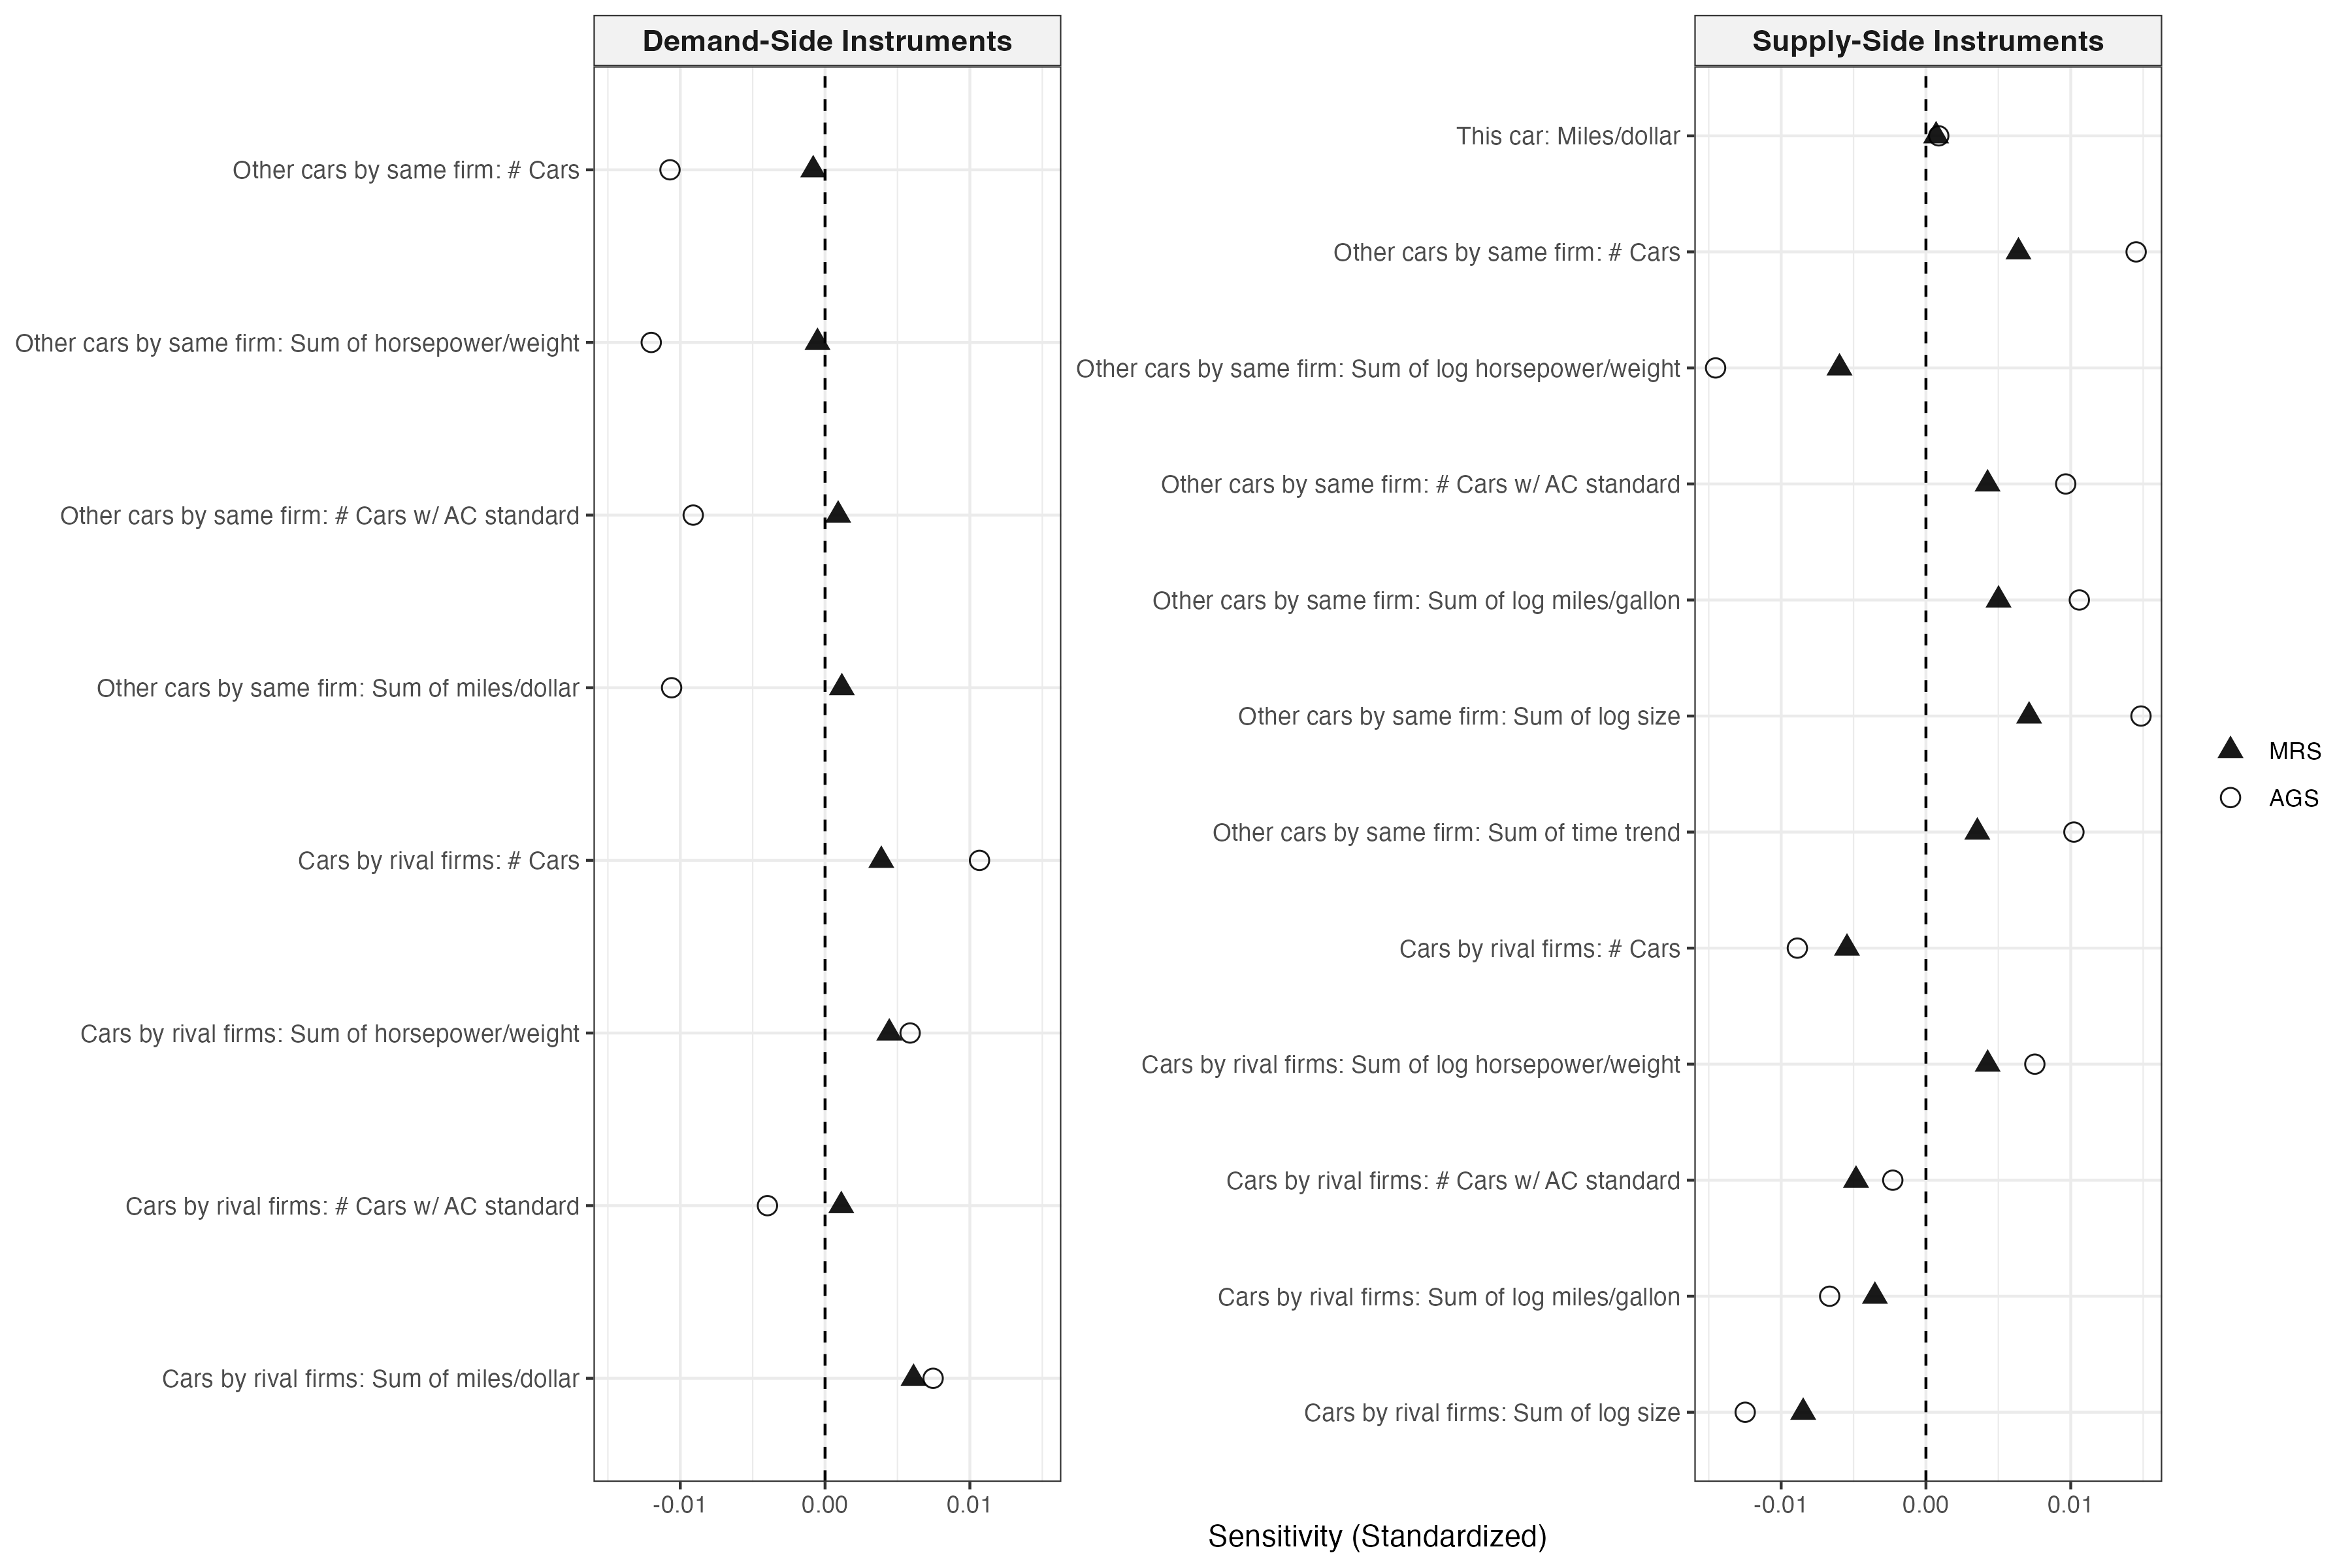
\includegraphics[height=0.7\textheight]{newBLP_replicated.png}
    \begin{itemize}
    	\item  AGS (hollow) vs.\ MRS (filled) for the average markup.
    	\item $\widehat\Delta_{markup}=0.56$.,  $J=345$ (p-value$<0.001$)
    \end{itemize}
\end{frame}

\begin{frame}{BPP: three weights, same moments}
    \centering
    {\small $35$ parameters, $q=325$, $n=1{,}765$, $J=538.7$ (df $290$).}
    \vspace{0.4em}
    \begin{tabular}{lcccccc}
        \toprule
             & \multicolumn{3}{c}{$\phi$ (permanent)} & \multicolumn{3}{c}{$\psi$ (transitory)} \\
        \cmidrule(lr){2-4}\cmidrule(lr){5-7}
             & Est. & SE & $\widehat\Delta$ & Est. & SE & $\widehat\Delta$ \\
        \midrule
        OMD  & $0.33$ & $0.043$ & $0.79$ & $0.07$ & $0.039$ & $0.79$ \\
        DWMD & $0.68$ & $0.113$ & $0.99$ & $0.03$ & $0.043$ & $0.99$ \\
        EWMD & $0.61$ & $0.109$ & $1.00$ & $0.00$ & $0.049$ & $1.00$ \\
        \bottomrule
    \end{tabular}
\end{frame}

\begin{frame}{BPP: efficiency vs.\ informativeness}
    \centering
    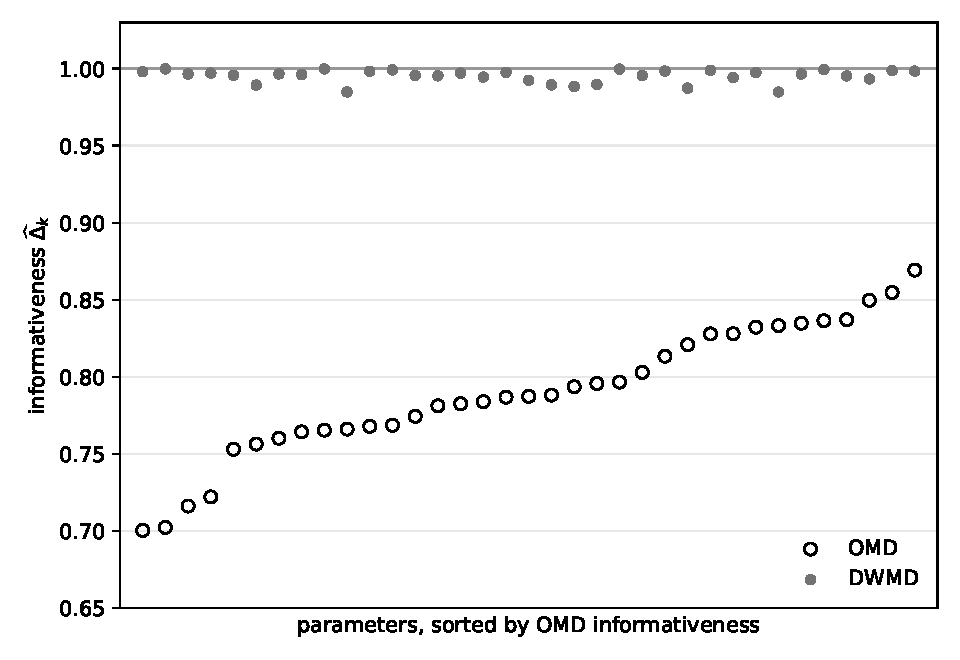
\includegraphics[height=0.73\textheight]{BPP_delta_weights.pdf}\\
    OMD $0.70$--$0.87$; \; DWMD $\approx 0.99$; \; EWMD $=1$. \quad
    SE($\phi$): $0.043\to0.113$.
\end{frame}

\begin{frame}{AJRY: income and democracy}
    \centering
    {\small Difference GMM, $n=127$ countries, df $44$; \;coefficient $\gamma$.}
    \vspace{0.5em}
    \begin{tabular}{lcccc}
        \toprule
        estimator & $\widehat\gamma$ & $J$ & $p$ & $\widehat\Delta_\gamma$ \\
        \midrule
        one-step (AB weight) & $-0.129$ & $71.3$ & $0.006$ & $0.93$ \\
        two-step efficient   & $-0.012$ & $61.4$ & $0.04$  & $0.81$ \\
        iterated fixed point & $-0.009$ & $45.3$ & $0.42$  & $0.77$ \\
        \bottomrule
    \end{tabular}
    \begin{itemize}
    	\item Efficient weight \alert{lowers} $\widehat\Delta_\gamma$: $0.93\to0.81\to0.77$.
    	\item $J$ stops rejecting (uncentered efficient weight).
		\item Sensitive to the choice of uncentered/centered efficient weight:
		\[J=45.3\,(p{=}0.42) \text{ vs }.\ J_c=70.4\,(p{=}0.007),
		\; J=J_c/(1+J_c/n). \]
    \end{itemize}
\end{frame}

\begin{frame}{AJRY: $J$ turns on a centering convention; $\Delta$ does not}
    \centering
    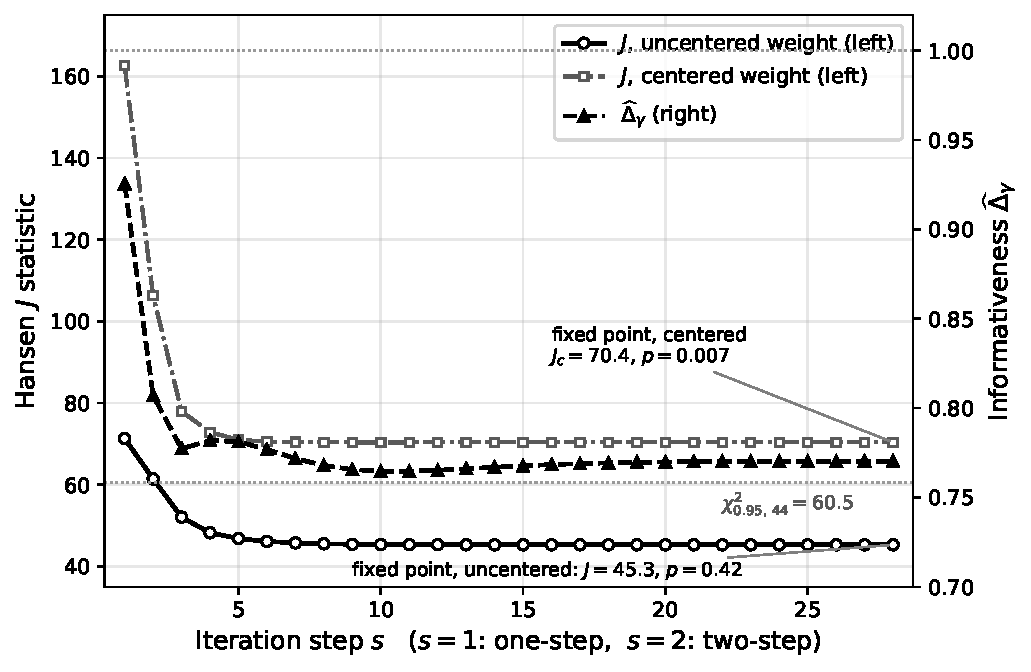
\includegraphics[height=0.75\textheight]{AJRY_J_vs_Delta.pdf}\\
    $\widehat\Delta_\gamma=0.77$, $J=45.3$, $J_c=70.4$,
\end{frame}

\begin{frame}{$J$ and $\Delta$ are complements}
    \centering
    \begin{tabular}{lccc}
        \toprule
             & $J$ under iteration & $\widehat\Delta$ under iteration & \\
        \midrule
        BLP  & flat at $345$    & $0.56\to0.24$ & $J$ silent, $\Delta$ falls \\
        BPP  & no iteration & $0.79/0.99/1$ & how to weight matters \\
        AJRY & $61.4\to45.3$    & $0.81\to0.77$ & $J$ verdict flips, $\Delta$ falls \\
        \bottomrule
    \end{tabular}
    \vspace{1.0em}
    \begin{itemize}\setlength{\itemsep}{0.5em}
        \item $J$: how far are the moments from zero?
        \item $\Delta$: how much of the variance do the moments explain?
    \end{itemize}
\end{frame}

% ============================================================ takeaways
\begin{frame}{Takeaways}
    \begin{enumerate}\setlength{\itemsep}{1.0em}
        \item Robust to misspecification: Evaluate sensitivity and informativeness \alert{at the pseudo-true
              value}
        \item Sensitivity rankings can reorder (BLP) 
        \item Weight choice in MD estimaiton is an efficiency--informativeness trade (BPP).
        \item Reporting $\widehat\Delta_k$ is straightforward if you calculate misspecification-robust standard
              errors: it is free and answers what the $J$-test cannot (AJRY).
    \end{enumerate}
\end{frame}

% ============================================================ appendix
\appendix

\begin{frame}{Appendix: Assumption 1 (regularity)}
    \hypertarget{jump:assum}{}
    \begin{enumerate}\footnotesize\setlength{\itemsep}{0.35em}
        \item[(i)]   $\{X_i\}_{i=1}^n$ i.i.d.
        \item[(ii)]  $\Theta\subset\mathbb R^p$ compact; unique interior
                     minimizer $\theta_0$ of the population objective.
        \item[(iii)] $g(X,\cdot)$ thrice continuously differentiable;
                     $\E\sup_\theta\|g\|^2,\,\E\sup_\theta\|G\|^2<\infty$, and
                     uniform $L^2$ ($L^1$) bounds on second (third) derivatives.
        \item[(iv)]  curvature matrices $A$ and $A+B$ nonsingular.
        \item[(v)]   (iterated GMM) the population updating map is a contraction
                     at $\theta_0$ \; ($\rho(-A^{-1}B)<1$).
        \item[(vi)]  weight conditions: \;
                     (a) one-step, $\widehat W\xrightarrow{p}W\succ0$,
                     $\sqrt n\,\vect(\widehat W-W)=n^{-1/2}\sum_i\omega_i+o_p(1)$; \;
                     (b) parameter-dependent, $\widehat\phi\xrightarrow{p}\phi_0$
                     asymptotically linear, $W(\phi)$ smooth with uniform
                     convergence of $\widehat W(\phi)$ and its derivative.
    \end{enumerate}
    \vfill
    {\footnotesize Return to:}\;
    \hyperlink{jump:p1}{\beamerreturnbutton{Prop 1}}\;
    \hyperlink{jump:p2}{\beamerreturnbutton{Prop 2}}\;
    \hyperlink{jump:p3}{\beamerreturnbutton{Prop 3}}\;
    \hyperlink{jump:p4}{\beamerreturnbutton{Prop 4}}
\end{frame}

\begin{frame}{Appendix: Notation}
    \hypertarget{jump:notation}{}
    \begin{itemize}\footnotesize\setlength{\itemsep}{0.45em}
        \item Primitives: \;
              $g=\E[g(X_i,\theta_0)]$, \quad
              $G=\E\!\big[\partial g(X_i,\theta_0)/\partial\theta'\big]$, \quad
              $W=\operatorname{plim}\widehat W$.
        \item Channels: \;
              $\nu_i=g(X_i,\theta_0)-g$, \quad
              $\gamma_i=\vect\big(G(X_i,\theta_0)'-G'\big)$, \quad
              $\omega_i=$ influence function of $\widehat W$, \quad
              $\psi^\phi=$ influence function of the first-step $\widehat\phi$.
        \item Curvature: \;
              $R=\E\!\big[\partial_{\theta'}\vect(G(X_i,\theta_0)')\big]$, \quad
              $H=(g'W\otimes I_p)R$, \quad $A=G'WG+H$.
        \item Iteration: \;
              $S=\partial_{\phi'}\vect W(\phi_0)$ (two-step) or
              $\partial_{\theta'}\vect W(\theta_0)$ (iterated), \quad
              $B=(g'\otimes G')S$.
        \item Coefficient maps: \;
              $M_\nu=-A^{-1}G'W$, \quad
              $M_\gamma=-A^{-1}(g'W\otimes I_p)$, \quad
              $M_\omega=-A^{-1}(g'\otimes G')$.
    \end{itemize}
    \vfill
    {\footnotesize Return to:}\;
    \hyperlink{jump:p1}{\beamerreturnbutton{Prop 1}}\;
    \hyperlink{jump:p3}{\beamerreturnbutton{Prop 3}}
\end{frame}

\begin{frame}{Appendix: AJRY multistart, common fixed point}
    \centering
    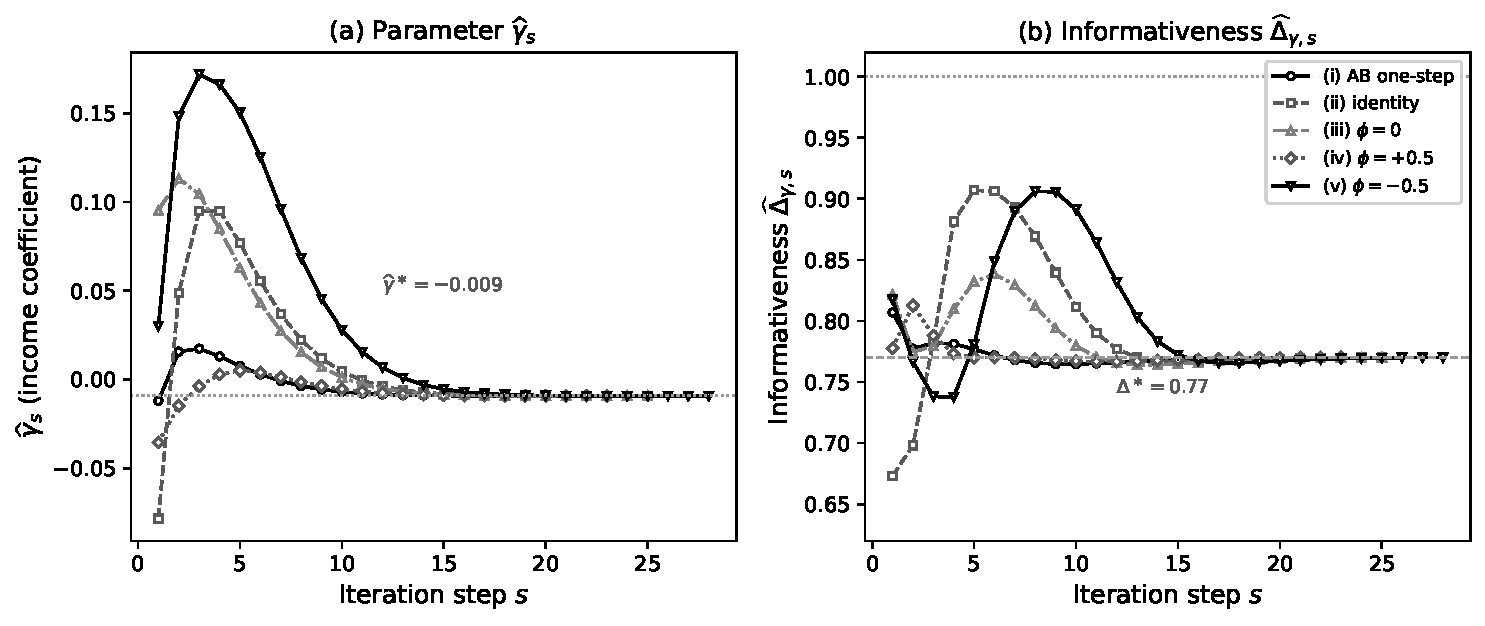
\includegraphics[height=0.66\textheight]{AJRY_multistart.pdf}\\
    {\small $\widehat\gamma_s$ and $\widehat\Delta_{\gamma,s}$ reach the common
    fixed point from every start; the approach of $\Delta$ is non-monotone.}
\end{frame}

\begin{frame}{Appendix: Schennach closed form}
    \centering
    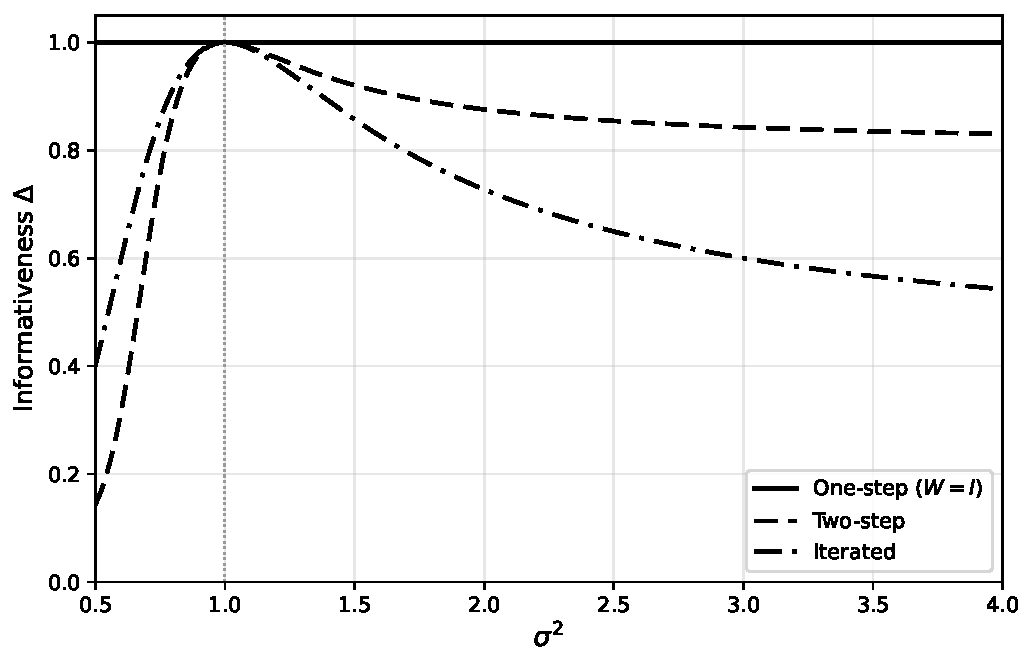
\includegraphics[height=0.62\textheight]{schennach_panel.pdf}\\
    {\small Schennach (2007, \textit{AoS}): normal mean with misspecified
    variance restriction; closed-form $\Delta$ for one-step, two-step, iterated, CUE.}
\end{frame}

\end{document}
